\chapter{RC 1}
%\lecture{3}{22 Sep. 18:30}{Temp}
\recitation{1}{29 Sep. 18:30}{}

\section{Review}
\subsection{Axioms of Probability}
A \textbf{probability space} is a triple \(\Omega,\mathcal{\MakeUppercase{f}},P\) that contains  
\begin{itemize}
	\item The \textbf{sample space} \(\Omega \) contains all possible outcome.  
	\item The \(\sigma\)-algebra \(\mathcal{\MakeUppercase{f}} \) is the \textbf{event space}. It is a subset of the power set of \(\Omega \) we are interested in. 
	\item The \textbf{probability measure} \(P\)
	
\end{itemize}
\subsection{Probability (measure)}
\begin{itemize}
    \item The \textbf{probability measure} \(P\) is a function \(P:\mathcal{\MakeUppercase{f}} \to [0,1] \) that satisfies the three axioms. 
	\begin{enumerate}
		\item \(P(\Omega ) = 1\) 
		\item Non-negative
		\item Countable additivity for disjoint sets in \(\mathcal{\MakeUppercase{f}} \).  
	\end{enumerate}
\end{itemize}
\subsection{\(\sigma\)-algebra }
\(\mathcal{\MakeUppercase{f}} \) is call a \(\sigma\)-algebra on a set \(\Omega \) If    
\begin{enumerate}
    \item \(\emptyset \in \mathcal{\MakeUppercase{f}} \)
    \item If \(A \in \mathcal{\MakeUppercase{f}} \implies A^c \in \mathcal{\MakeUppercase{f}} \) 
    \item If \(A_1, A_2, \dots \in \mathcal{\MakeUppercase{f}} \), then \(\cup_{i = 1} A_i \in \mathcal{\MakeUppercase{f}}\) 
\end{enumerate}
\begin{eg}
    Let \(\Omega  = \{1,2,3,4,5,6\}\), find a minimal* \(\sigma\)-algebra that contains the sets \(\{1,2,3\},\{1\}\)  
\end{eg}
    Answer: \footnote[1]{\(\mathcal{\MakeUppercase{F}} =  \{\emptyset,\Omega ,\{1\},\{1,2,3\},\{4,5,6\},\{2,3,4,5,6\},\{2,3\},\{1,4,5,6\}\}\) }

\subsection{Conditional Probability}
For the general definition, take events \(A, B,\quad\) and assume that \(P(B) > 0\). The \textit{conditional probability} of the event \(A\) given \(B\) equals 
\[
    P(A|B) = \frac{P(A\cap B)}{P(B)}
\]
TBD (an example)
\subsection{Independence}
Events \(A_1,\dots,A_n\) are independent if 
\[
    P(\cap_{i = 1}^n A_i) = \prod_{i=1}^nP(A_i)
\]
Please note that it means you can not just check \(P(A_i\cap A_j) = P(A_i)P(A_j), i \neq j\). One example is teh following 
\begin{eg}[Pairwise Independence but not independent variables]
(\cite{IntroPanchenko} Exercise 1.4.2) Consider a regular tetrahedron die painted
blue, red and green on three sides and painted in all three
colours on the fourth side. If the die is equally likely to land
on any side, show that the appearances of these colours on
the side it lands on are pairwise-independent but not independent.
\end{eg}
\section{Problem}
\textbf{Problem 1.} Put $r$ distinguishable balls into $n$ different boxes. What is the probability of all $n$ boxes are occupied?\\ \\
\textit{Probabilistic approach.} $A_i=\{\text{Box $i$ is occupied}\}$ for all $i=1,\cdots, n$.
\begin{equation}
\mathbb{P}(\text{No empty boxes}) = \mathbb{P}\Big(\bigcup_{i=1}^n A_i\Big).
\end{equation}
(Inclusion-exclusion principle!)\\ \\
\textit{Combinatorial approach.} Define $A(r,n)$ as the number of distributions such that all $n$ boxes are non-empty when you put $r$ balls into them. Then the probability is $A(r,n)/n^r$. Knowing $A(r,n+1)$ can lead us to $A(r,n)$:
\begin{equation}
A(r,n) = \sum_{k=1}^{r-1}A(r-k,n-1).
\end{equation}
Knowing this, we can prove that:
\begin{equation}
A(r,n) = \sum_{\nu = 0}^n(-1)^\nu\binom{n}{\nu}(n-\nu)^r.
\end{equation}
(Use Induction!)\\ \\
\textit{(Think about it!)} What is the probability of exactly $m$ boxes are occupied?
\begin{equation}
\text{number of distributions }= \binom{n}{m}\times A(r,m).
\end{equation}
$A(r,m) = \mathbb{P}(\text{$r$ balls into $m$ boxes and all of the boxes are occupied})\times m^r$.

%\begin{figure}[h]
%    \centering
%    \includegraphics[width=\textwidth]{Figures/rc1_f1_1.png}
%    \includegraphics[width=\textwidth]{Figures/rc1_f1_2.png}
%    \label{fig:rc1_1}
%\end{figure}
\begin{figure}[h]
    \centering
    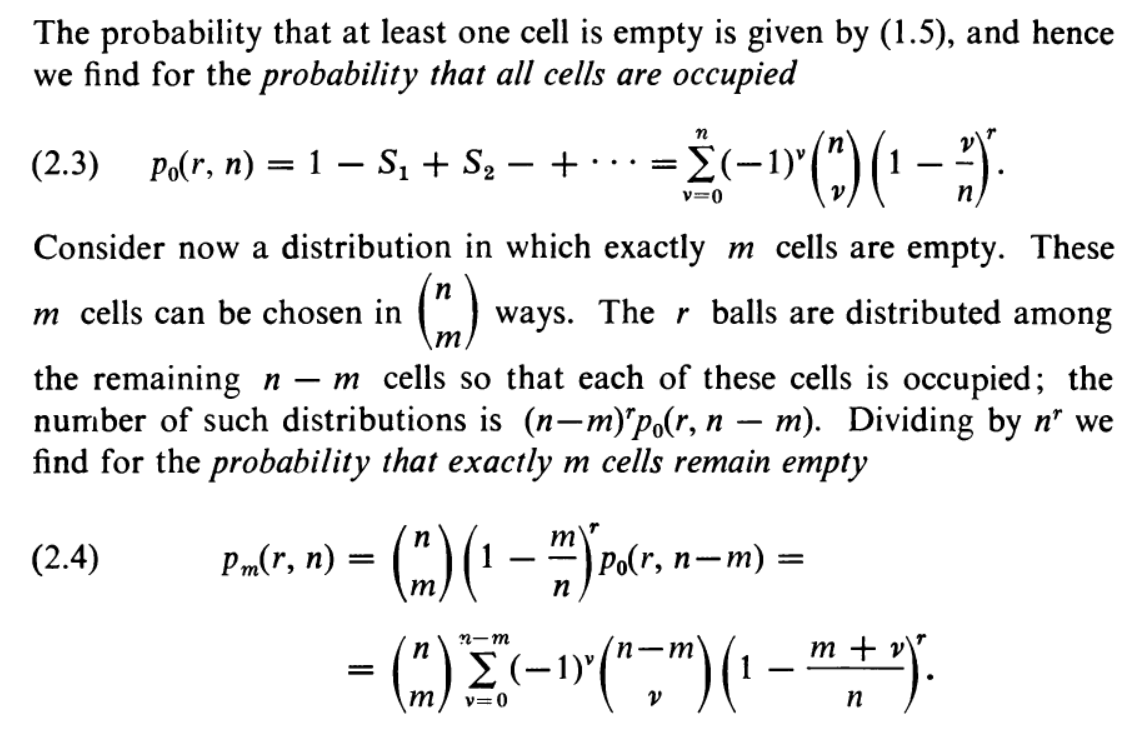
\includegraphics[width=\textwidth]{Figures/rc1_f2.png}
    \caption{A problem in Feller}
    \label{fig:rc1_2}
\end{figure}
